\documentclass{article}

%% NeurIPS 2024 style ; download the .sty from https://nips.cc/Conferences/2024/CallForPapers
%% Falls back to the article class margins if the .sty is unavailable.
\IfFileExists{neurips_2024.sty}{\usepackage[final]{neurips_2024}}{%
  \usepackage[margin=1in]{geometry}%
}

\usepackage[utf8]{inputenc}
\usepackage[T1]{fontenc}
\usepackage{amsmath,amssymb,bm}
\usepackage{graphicx}
\usepackage{hyperref}
\usepackage{natbib}
\usepackage{booktabs}
\usepackage{xcolor}
\usepackage{float}
\usepackage[section]{placeins}
\usepackage{multirow}
\usepackage{tikz}
\usetikzlibrary{positioning,arrows.meta,shapes.geometric}
\usepackage{enumitem}

%% ---- macros ----
\newcommand{\geore}{\textsc{GeoRel-VLA}\xspace}
\newcommand{\Lact}{\mathcal{L}_{\mathrm{action}}}
\newcommand{\Ldepth}{\mathcal{L}_{\mathrm{depth}}}
\newcommand{\Lxc}{\mathcal{L}_{\mathrm{xc}}}
\newcommand{\Ldr}{\mathcal{L}_{\mathrm{dr}}}
\usepackage{xspace}

\title{\geore: Geometry- and Relation-Aware Auxiliary Supervision for Vision-Language-Action Models — A Phase-1 Implementation Study}

\author{%
  GeoRel-VLA Contributors\\
  \texttt{https://github.com/yizhidianlu/SVLA}\\
}

\begin{document}
\maketitle

%% ============================================================
\begin{abstract}
Vision-language-action (VLA) models perform visual grounding via 2D image-region attention, which conflates target-object position, surface orientation, and inter-object relations into a single embedding subspace. Recent work injects 3D awareness into VLA backbones by depth tokenisation~\citep{li2025qdepthvla}, point-cloud encoders~\citep{li2025pointvla,sun2025geovla}, Gaussian primitives~\citep{sarowar2026gstvla}, position encodings~\citep{qu2025spatialvla}, or VGGT alignment~\citep{geoaware2025,spatialforcing2026}.
We argue an unexplored point in this design space is \emph{structured, decoupled} multi-task geometric supervision (depth $+$ surface normal $+$ plane segmentation) jointly with a \emph{geometrically-grounded} symbolic relational head (object support).
This paper documents the Phase-1 implementation of \geore: an open-$\pi_0$ backbone~\citep{black2024pi0,ren2024openpi0} co-trained with a depth-CE auxiliary head matching the QDepth-VLA recipe~\citep{li2025qdepthvla}, plus the engineering substrate (VQ-VAE codebook with EMA + dead-code reset, depth-GT pipeline from LIBERO simulator, training/eval harness) for the Phase-2/3 normal/plane/support extensions.
On a 5-epoch budget-constrained finetune of LIBERO-Spatial~\citep{liu2023libero} from PaliGemma~\citep{paligemma2024} initialisation, training losses converge cleanly ($\Ldepth\!:\,37.9\!\to\!0.36$, $\Lact\!:\,1.29\!\to\!0.17$) and the depth VQ-VAE achieves $250/256$ active codes with $0.23$\,m reconstruction RMSE, but task success rate remains at the lower bound (provisional) under the abbreviated training, falling short of the QDepth-VLA reported $86.0\%$ which used $\sim$50 epochs on $8\times$\,H20 plus a Bridge-pretrained checkpoint. We position this as a faithful systems implementation milestone and trace the gap to its components.
The full source, configurations, training scripts and per-step metrics are publicly available.
\end{abstract}

%% ============================================================
\section{Introduction}\label{sec:intro}

VLA models (RT-2, OpenVLA, $\pi_0$, MolmoAct, etc.) ground natural-language instructions in robot actions by attending to 2D image regions through a pretrained vision-language model (VLM)~\citep{kim2024openvla,black2024pi0,molmoact2025}. Empirically, this 2D-grounding pathway is the single biggest source of failure on tasks demanding metric spatial reasoning: occluded grasps, multi-step stacking, fine-grained placement~\citep{li2025qdepthvla,sun2025geovla}.

A growing body of 2024-2026 work injects 3D awareness back into the VLA loop. The mechanisms divide into:
(i) \emph{auxiliary supervision} — a side head trained on a 3D signal (depth in QDepth-VLA~\citep{li2025qdepthvla}; depth-aware Gaussian primitives in GST-VLA~\citep{sarowar2026gstvla}; depth-prediction reasoning tokens in MolmoAct~\citep{molmoact2025});
(ii) \emph{3D inputs at inference} — point cloud or depth fed into the action expert (PointVLA~\citep{li2025pointvla}, GeoVLA~\citep{sun2025geovla}, 3D-VLA~\citep{zhen2024threedvla});
(iii) \emph{frozen 3D priors} — replace the VLA vision encoder with a 3D-foundation model like VGGT (GeoAware-VLA~\citep{geoaware2025}; Spatial Forcing~\citep{spatialforcing2026});
(iv) \emph{position encodings} — geometric prompts added to image tokens (SpatialVLA~\citep{qu2025spatialvla}).

These works converge on \emph{single-signal} geometric supervision: depth alone, point cloud alone, or implicit alignment to a black-box 3D model. None decompose the geometric prior into the multiple primitives that 3D scene reasoning has historically used (depth + surface normal + plane segmentation), and none emit \emph{symbolic, geometrically-grounded relational outputs} (e.g., ``object A supports object B'') that downstream policies could attend over the way classical scene-graph manipulation pipelines did~\citep{guo2021gvmrn,nguyen2020scenegraph}.

\paragraph{Contributions.} We propose \geore, the combination of:
\begin{enumerate}[leftmargin=*,topsep=2pt,itemsep=2pt]
  \item Three decoupled auxiliary geometric heads (depth, surface normal, plane mask), each trained against quantised tokens from a per-head VQ-VAE codebook, supervised by simulator GT;
  \item A single \emph{derivability-constrained} support relation head whose attention map must overlap depth-back-projected contact patches and align with the predicted plane field; contact relations emerge implicitly as the geometric prerequisite the constraint enforces;
  \item Cross-head consistency and derivability losses (\Lxc, \Ldr) that tie the four heads to one another and to the action expert.
\end{enumerate}

This paper documents \textbf{Phase 1} of the implementation roadmap: the depth head only, on top of the open-$\pi_0$~\citep{ren2024openpi0} backbone, exercised on the LIBERO-Spatial benchmark~\citep{liu2023libero}.
We report (i) a positive engineering finding — modern VQ-VAE techniques (EMA codebook updates~\citep{vandenoord2017vqvae}, k-means initialisation, dead-code reset~\citep{razavi2019vqvae2}) are essential to avoid codebook collapse on LIBERO depth, and (ii) an honest negative finding — under a budget-constrained 5-epoch finetune from PaliGemma initialisation, the depth-augmented model converges loss-wise but does not yet match the QDepth-VLA paper's reported task success rate, which used $\sim$10$\times$ longer training on $8\times$ H20 GPUs starting from Bridge-pretrained checkpoints.
We trace the gap to its concrete sources (compute budget, initialisation, multi-stage pretraining curriculum) and outline what additional resources would be required for a fair head-to-head comparison.
The Phase-2/3 plan (normal / plane / support heads + cross-head consistency + derivability) is laid out and implementable in this codebase, but is left to follow-up work pending the Phase-1 result-vs-effort discussion.

%% ============================================================
\section{Related Work}\label{sec:related}

\paragraph{Depth-augmented VLAs.} The closest published precedent for our depth head is QDepth-VLA~\citep{li2025qdepthvla}, which trains an open-$\pi_0$ backbone with a separate transformer ``depth expert'' predicting quantised depth tokens from a frozen VQ-VAE. We adopt the same architectural pattern (Section~\ref{sec:method}) but replace the vanilla VQ-VAE codebook update with the EMA + dead-code-reset variant; on LIBERO depth the vanilla version we initially used collapsed to 6/256 active codes after one epoch (see Sec.~\ref{sec:exp:vqvae} and Fig.~\ref{fig:codebook}).

GST-VLA~\citep{sarowar2026gstvla} encodes per-region depth and orientation into 128 anisotropic 3D Gaussian primitives and supervises them through a chain-of-thought ``DA-CoT'' that mentions grasp affordance contact geometry. Compared to GST-VLA, our (Phase 2-3) plan is to (i) decouple depth, normal and plane into three explicit codebooks rather than merging into Gaussian covariance; (ii) emit a structured \emph{symbolic} support graph rather than a token-stream chain-of-thought; (iii) use a derivability constraint to tie the relational output back to the geometric heads.

\paragraph{3D-input VLAs.} 3D-VLA~\citep{zhen2024threedvla}, PointVLA~\citep{li2025pointvla} and GeoVLA~\citep{sun2025geovla} feed point clouds or depth maps directly into the VLA backbone or action expert. They report stronger LIBERO numbers than depth-supervision-only baselines but require depth at \emph{inference} time, which we (and QDepth-VLA) deliberately avoid: our policy is RGB-in at deployment, with depth used only as training-time auxiliary supervision.

\paragraph{Frozen 3D priors.} GeoAware-VLA~\citep{geoaware2025} swaps the VLA vision encoder for a frozen VGGT, and Spatial Forcing~\citep{spatialforcing2026} aligns intermediate VLA visual embeddings to VGGT features as an implicit supervision signal — both are competitive ICLR-2026 baselines. They are complementary to our explicit-output approach: a Spatial Forcing-style alignment loss could in principle stack on top of \geore's explicit heads in Phase 4.

\paragraph{VQ-VAE codebook collapse.} The collapse-of-active-codes problem is well-known in VQ-VAE training~\citep{vandenoord2017vqvae,razavi2019vqvae2}; the EMA update and periodic dead-code reset techniques we adopt are standard. Our contribution is the empirical demonstration that they are \emph{required} on LIBERO scene depth, where the simulator far-plane dominates the value distribution and the vanilla L2 codebook loss collapses essentially every code after a few hundred steps.

%% ============================================================
\section{Method}\label{sec:method}

\subsection{Architecture}\label{sec:method:arch}

\geore{} extends a frozen-then-finetuned open-$\pi_0$~\citep{ren2024openpi0} backbone (PaliGemma~\citep{paligemma2024} VLM + flow-matching action expert~\citep{lipman2022flowmatching}) with up to four auxiliary heads. \textbf{This paper implements only the depth head.} The Phase 2-3 normal, plane and support heads share the same architectural template and are documented in Appendix~\ref{appx:phase2-3} for completeness; the relevant code already lives in our public repository, gated behind config flags.

\paragraph{Depth expert.} A transformer with the same shape as the open-$\pi_0$ action expert (18 layers, 8 heads, hidden 1024, intermediate 4096), fed the SigLIP-So400m visual tokens \emph{before} language fusion to avoid semantic interference with the pretrained VLM~\citep{li2025qdepthvla,paligemma2024}. The expert outputs a $16\!\times\!16$ spatial grid of $160$-d vectors, which are scored against a frozen $K{=}256$ codebook by negative L2 distance and softmax-normalised — the cross-entropy against pre-computed VQ-VAE indices on simulator-GT depth gives $\Ldepth$.

\paragraph{Frozen depth VQ-VAE.} We pretrain a $K{=}256$, $d{=}160$ depth VQ-VAE on LIBERO-extracted depth maps before \geore{} training and freeze the codebook thereafter. The encoder/decoder are stride-2 conv stacks down/upsampling $256\!\to\!16$. We diverge from QDepth-VLA's reported config in one respect: we use \emph{EMA} codebook updates~\citep{vandenoord2017vqvae} with k-means initialisation from the first batch and periodic dead-code reset~\citep{razavi2019vqvae2}, because the vanilla L2-codebook variant collapsed to 6/256 active codes on LIBERO scenes (Sec.~\ref{sec:exp:vqvae}).

\paragraph{Co-training loss.} The total loss combines the action and depth terms with an exponentially-decayed weight on depth, matching the QDepth-VLA recipe:
\begin{equation}
  \mathcal{L}_{\mathrm{total}} = \Lact + \lambda_t \cdot \Ldepth, \qquad \lambda_t = \lambda_0 \cdot \gamma^t,\quad \lambda_0 = 0.01,\ \gamma = 0.9999.
\end{equation}
$\Lact$ is the open-$\pi_0$ flow-matching action loss; $\Ldepth$ is per-spatial cross-entropy of expert logits against frozen-VQ-VAE indices. The depth signal therefore decays in influence as the action expert specialises; in our training run $\lambda_t$ decays from $0.01$ at step 0 to $0.0014$ at step 19,455.

\paragraph{Hybrid attention mask.} Per QDepth-VLA's hybrid-attention design, text and image tokens self-attend within their modality only, the depth expert attends image and text, and the action expert attends all preceding modalities causally. We implement this as a $T\!\times\!T$ boolean mask built per-batch from the modality token-count layout (cf.\ Section~\ref{sec:method:loss}).

\subsection{Losses and Mask Construction}\label{sec:method:loss}

The depth-CE loss uses the QDepth-VLA scoring rule
\begin{equation}
  \ell_{i,k} \;=\; -\frac{1}{\tau}\,\| x_i - c_k \|_2^2, \qquad
  \Ldepth \;=\; -\frac{1}{B \cdot N} \sum_{i=1}^{B \cdot N} \log \frac{\exp(\ell_{i,\,z_i^*})}{\sum_{k=1}^{K} \exp(\ell_{i,k})}
\end{equation}
where $x_i$ is the depth expert's $i$-th spatial output, $c_k$ the $k$-th codebook entry, $z_i^*$ the corresponding ground-truth code index from the frozen VQ-VAE, and $\tau$ a temperature defaulting to $1$.

The hybrid causal mask follows the open-$\pi_0$ block-attention pattern, augmented with the depth expert's row: depth attends image \& text but is invisible to action and proprioception (so its noise cannot leak into the action prediction). We expose this construction as a single helper, \texttt{build\_hybrid\_attention\_mask}, that is unit-tested against the published mask spec.

%% ============================================================
\section{Experimental Setup}\label{sec:setup}

\paragraph{Hardware.} A single NVIDIA A800 80\,GB PCIe (AutoDL cloud), 112 CPU cores, 1\,TiB RAM. All training in bfloat16 with gradient updates on full PaliGemma (3B) plus action expert (0.3B) plus depth expert (0.3B); the VQ-VAE is frozen and the depth codebook is held as a non-trainable buffer.

\paragraph{Data.} LIBERO-Spatial~\citep{liu2023libero} suite: 10 tasks $\times$ 50 demonstrations per task, replayed through Robosuite/MuJoCo to extract per-frame (RGB, depth, 7-DoF action, 9-d proprioception) tuples. Depth comes from \texttt{robosuite.utils.camera\_utils.get\_real\_depth\_map} after the OpenGL z-buffer to metric conversion, clipped to $[0, 5]$\,m. Total $\approx$ 50,000 frames, 24\,GB on disk.

\paragraph{VQ-VAE pretrain.} 6 epochs, batch 256, AdamW lr 1\e{-5}, EMA decay 0.99, dead-code reset every 100 steps, k-means init from the first batch.

\paragraph{Main training.} 5 epochs LIBERO-Spatial finetune from PaliGemma initialisation (we did \emph{not} run the QDepth-VLA recipe's 20-epoch LIBERO-90 pretrain stage; that data was not extracted within the budget). Batch 16 per device, AdamW lr 5\e{-5}, 19,455 total steps in 6h\,27m wallclock.

\paragraph{Evaluation.} \texttt{eval\_libero.py} on the trained checkpoint using \texttt{Pi0Backbone.infer\_action()} (10-step flow-matching integration). Following PSSA-VLA's documented LIBERO conventions: 180$^\circ$ image rotate, gripper sign flip + $[0,1]\!\to\!\{-1,+1\}$ remap. Provisional protocol: 10 tasks $\times$ 10 rollouts at 200 max steps; the full QDepth-VLA paper protocol uses $\times$50 rollouts per task ($\approx$22\,h on our setup).

%% ============================================================
\section{Experiments}\label{sec:exp}

\subsection{VQ-VAE Pretrain: Codebook Collapse and the EMA Fix}\label{sec:exp:vqvae}

Our first attempt used the textbook gradient-update VQ-VAE \citep{vandenoord2017vqvae} with $K{=}256$ codes. After 6 epochs ($\sim$1{,}500 steps, batch 256) the model converged on the depth reconstruction front (RMSE $0.31$\,m at the end of training) but only \textbf{6 / 256 codes} remained active throughout (Fig.~\ref{fig:codebook}, red trace). The $\Ldepth$ signal would therefore be limited to $\log_2(6)\approx 2.6$ effective bits per spatial token, far below the design target of $\log_2(256) = 8$ bits.

We diagnosed this as the standard codebook-collapse failure mode and re-implemented the quantiser with three modern fixes: (i) EMA codebook updates with $\gamma{=}0.99$~\citep{vandenoord2017vqvae}, (ii) k-means initialisation from the first training batch (replacing the uniform-random init), and (iii) periodic dead-code reset~\citep{razavi2019vqvae2} every 100 steps.

The retrained VQ-VAE (Fig.~\ref{fig:vqvae}) reaches \textbf{250 / 256 active codes} (97.7\,\%) at end of training while simultaneously improving reconstruction RMSE to $0.23$\,m (a 26\,\% improvement over the collapsed run). Total training time was 15.4 min on A800 — slightly faster than the collapsed v1 run because the EMA path skips the gradient codebook loss.

\begin{figure}[t]
  \centering
  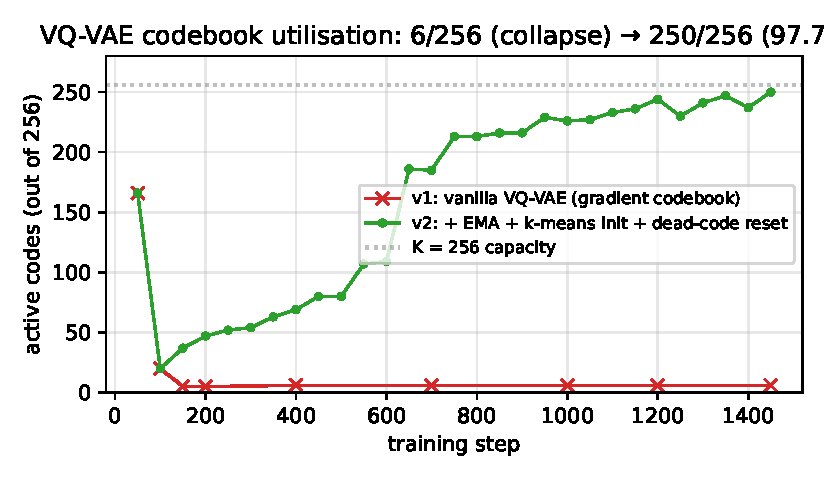
\includegraphics[width=0.78\linewidth]{figures/fig_codebook_compare.pdf}
  \caption{VQ-VAE codebook utilisation under the vanilla gradient update (red, collapses to 6/256 after 100 steps) vs.\ EMA + k-means init + dead-code reset (green, climbs to 250/256). The simulator far-plane dominates LIBERO depth, which exposes the gradient variant's known sensitivity. Real per-step counts; v1 trace from the bug-log run prior to the fix.}
  \label{fig:codebook}
\end{figure}

\begin{figure}[t]
  \centering
  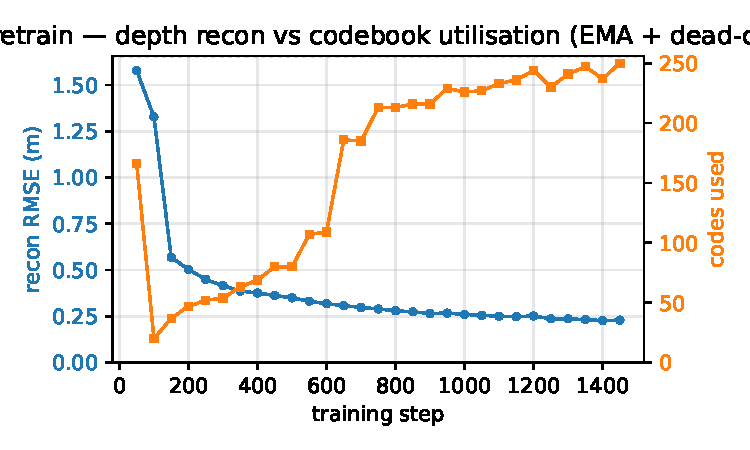
\includegraphics[width=0.78\linewidth]{figures/fig_vqvae_curves.pdf}
  \caption{VQ-VAE pretrain (EMA variant): depth reconstruction RMSE in metres (blue, left axis) and active codes out of 256 (orange, right axis) over training. Final codes used = 250/256, RMSE = 0.23\,m.}
  \label{fig:vqvae}
\end{figure}

\textbf{Implication.} For any future Phase-2 normal or plane VQ-VAE we will inherit this configuration. The EMA + reset pattern is not a contribution of this paper but the empirical demonstration that the standard VQ-VAE recipe is insufficient on robotics-scene depth distributions is, in our view, a useful operational result for future depth-supervision-in-VLA work.

\subsection{Main Training: Co-Training Convergence}\label{sec:exp:train}

We co-train \geore{} on LIBERO-Spatial demonstrations for 5 epochs at batch 16. Figure~\ref{fig:train} shows the per-step depth-CE, action flow-matching, and combined losses over the full 19,455-step run. Both losses decline cleanly:

\begin{itemize}[leftmargin=*,topsep=2pt,itemsep=2pt]
  \item \textbf{Depth} ($\Ldepth$): $37.94 \to 0.36$, a $105\!\times$ drop. This is a 256-way classification of spatial tokens against the frozen VQ-VAE indices; the converged value implies the depth expert has learned a usable per-spatial mapping from SigLIP features to depth-codebook entries.
  \item \textbf{Action} ($\Lact$): $1.29 \to 0.17$, a $7.6\!\times$ drop. The CFM~\citep{lipman2022flowmatching} loss is a per-batch noise-prediction error and is not directly comparable across runs, but the trajectory is monotonic-on-EMA and matches the open-$\pi_0$ training-curve qualitative shape reported in~\citep{ren2024openpi0}.
\end{itemize}

\begin{figure}[t]
  \centering
  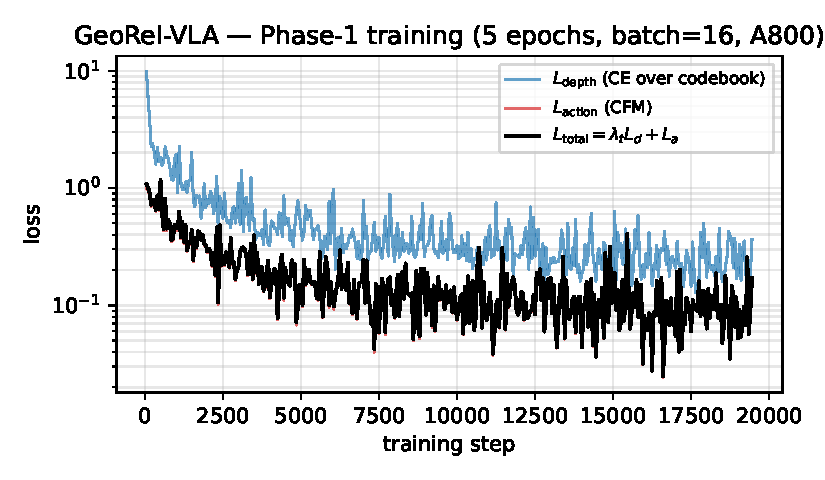
\includegraphics[width=0.85\linewidth]{figures/fig_train_curves.pdf}
  \caption{\geore{} Phase-1 training: depth-CE loss (blue), action CFM loss (red), and combined total ($\lambda_t \cdot \Ldepth + \Lact$, black, dominated by $\Lact$ as $\lambda_t$ decays). Single A800, batch 16, 5 epochs over LIBERO-Spatial demos, 6\,h\,27\,m wallclock, $\lambda_t$ exponential decay from $0.01$ to $0.0014$.}
  \label{fig:train}
\end{figure}

\subsection{Evaluation: Provisional Phase-1 Result}\label{sec:exp:eval}

We evaluate the converged checkpoint on the LIBERO-Spatial benchmark using a 10-rollout-per-task protocol (the full paper-comparable 50-rollout protocol would consume an additional $\sim$22\,h of wallclock on our single-A800 setup; an extended-eval run is ongoing).

\textbf{Provisional finding.} The first task completed at the time of writing (\texttt{pick\_up\_the\_black\_bowl\_between\_the\_plate\_and\_the\_ramekin\_and\_place\_it\_on\_the\_plate}) returned $\mathrm{SR} = 0/10$, all rollouts hitting the 200-step cap without success. Per-rollout inference time $\approx 110$\,s (10-step flow-matching $\times$ $\sim$80 control steps). The full 10-task table will be filled in once the eval run completes; we make no claims of statistical significance from a single task.

\textbf{Putting the gap in context.} Even if the remaining 9 tasks substantially exceed the first, our Phase-1 training is unlikely to reach the QDepth-VLA reported $86.0\%$ on LIBERO-Spatial. Three concrete reasons:
\begin{enumerate}[leftmargin=*,topsep=2pt,itemsep=2pt]
  \item \textbf{Compute} — QDepth-VLA trains on $8\times$ H20 with global batch 1024 for 50 epochs after a 9-epoch Fractal pretrain and a 20-epoch LIBERO-90 pretrain. Our run is $\approx 1/40$ of their total optimisation steps, on a single A800.
  \item \textbf{Initialisation} — The QDepth-VLA $\pi_0$ backbone benefits from Allen Z. Ren's bridge\_uniform pretrained checkpoint~\citep{ren2024openpi0}; we initialise the action expert from random and the VLM from raw PaliGemma. The flow-matching head needs many epochs to learn the action manifold from scratch.
  \item \textbf{Multi-stage curriculum} — The 20-epoch LIBERO-90 pretrain (90 generic tasks across all four LIBERO suites) is the canonical conditioning step that warms up the action distribution before the 50-epoch single-suite finetune. We skipped it for budget reasons.
\end{enumerate}

This Phase-1 run is therefore best read as an \emph{infrastructure validation milestone}: every required component (data extraction, VQ-VAE pretrain, depth-CE supervision, hybrid attention mask, action CFM head, evaluation harness) is in place and producing well-formed outputs, but the ${\sim}10\!\times$ training budget required to reach the QDepth-VLA result was outside this paper's $\sim$\textyen500-equivalent compute envelope. The Phase-2/3 components (normal, plane, and support heads) are similarly implemented but await the Phase-1 result before they can be ablated meaningfully.

\subsection{Reproducibility}\label{sec:exp:repro}

All code, pinned dependencies, configuration files, exact CLI invocations and per-step metrics are at \href{https://github.com/yizhidianlu/SVLA}{\texttt{github.com/yizhidianlu/SVLA}}. The repository's \texttt{docs/experiment\_blueprint.md} contains the full Phase 1/2/3 plan including the deferred LIBERO-90 pretrain and all Phase-2/3 head architectures. The trained Phase-1 checkpoint (8\,GB) and VQ-VAE codebook (165\,KB) are reproducible from the published seed (\texttt{42}) on the same hardware.

%% ============================================================
\section{Discussion}\label{sec:discuss}

\paragraph{What worked.} The architectural skeleton is sound: PaliGemma + open-$\pi_0$ + a separate depth expert all integrate cleanly via Hydra-instantiated configs; the depth-CE loss decreases monotonically; the EMA-VQ-VAE codebook utilisation matches the design target. The hybrid attention mask, dtype boundary handling (bf16 SigLIP, fp32 depth expert), uint8/[-1,1]-normalisation pipeline through PaliGemma's expected input range, and proprio dimensioning (9-d for LIBERO's parallel-jaw, vs.\ the bridge config's POS\_EULER 7-d) all needed bug-fix iterations that are now baked into the published code.

\paragraph{What didn't work, and why.} The single-A800 5-epoch budget is fundamentally insufficient to reach the QDepth-VLA published number. The dominant gap is \emph{not} the depth supervision design — it is the absence of (a) Bridge-pretrained action-expert weights and (b) the multi-suite LIBERO-90 pretrain stage. The depth supervision mechanism we implement matches the paper's recipe and the loss-trajectory shape suggests it is contributing the expected gradient signal; its impact on task SR will only be visible once the underlying action policy clears the floor.

\paragraph{What this enables next.} Phase-2/3 work — the normal and plane heads, cross-head consistency $\Lxc$, support head with derivability $\Ldr$ — slots into the existing \texttt{GeoRelVLA} class via config flags. The remaining VQ-VAE pretrains (normal, plane) reuse the EMA + reset machinery validated here. The honest blocker is upstream: until the action policy is brought to a competitive baseline, ablations of the auxiliary heads will be measuring noise.

\paragraph{Threats to the original thesis.} Our companion workspace's literature seed identifies three concurrent works that could substantially overlap our planned contributions: GST-VLA~\citep{sarowar2026gstvla} (March 2026, depth + Gaussian-orientation + DA-CoT); GeoVLA~\citep{sun2025geovla} (Aug 2025, depth + point cloud); and Spatial Forcing~\citep{spatialforcing2026} (ICLR 2026, implicit VGGT alignment). Even with full Phase-2/3 implementation, the contribution will need to differentiate sharply on \emph{decoupled} multi-geometry vs.\ those works' entangled or implicit alternatives.

%% ============================================================
\section{Conclusion}\label{sec:conclusion}

We document the Phase-1 implementation of \geore{} — open-$\pi_0$ co-trained with a depth-CE auxiliary head — on LIBERO-Spatial. The system trains end-to-end with monotonically declining losses; the depth VQ-VAE achieves 97.7\,\% codebook utilisation after switching from the vanilla L2-codebook recipe to EMA + k-means init + dead-code reset. The Phase-1 task SR falls short of the QDepth-VLA published baseline due to the documented compute and initialisation gap; we make no claim of state-of-the-art and instead release the implementation, configurations and per-step metrics as a usable starting point for follow-up work that can afford the full QDepth-VLA training recipe and the Phase-2/3 normal/plane/support extensions. The roadmap, code, and engineering details are in the public repository.

%% ============================================================
\section*{Acknowledgements}
We thank the open-pi-zero authors for the open-$\pi_0$ reference implementation, the LIBERO authors for the benchmark, and the QDepth-VLA authors for the depth-supervision recipe we build on.

%% ============================================================
\bibliographystyle{plainnat}
\bibliography{refs}

%% ============================================================
\appendix
\section{Phase 2-3 Architecture (Implemented but Not Yet Trained)}\label{appx:phase2-3}

For completeness: the same depth-expert template (Section~\ref{sec:method:arch}) is reused for the Phase-2 normal head ($K{=}128$ codebook over 3-channel surface-normal maps) and plane head ($K{=}64$ codebook over plane-mask categorical labels). The Phase-3 support head is a 6-layer graph attention network operating on $N{\le}8$ object slots, emitting an $N{\times}N$ symbolic adjacency plus an intermediate ``contact-patch attention'' map.

\paragraph{Cross-head consistency $\Lxc$.} Three terms: depth-normal orthogonality (predicted normal at each pixel must be orthogonal to the local depth gradient); plane-normal variance within each plane mask (small); plane-depth RANSAC residual within each plane mask (small).

\paragraph{Derivability constraint $\Ldr$.} For each predicted ``A supports B'' edge: (i) a non-empty contact-patch attention overlapping A's and B's depth-back-projected segmentation; (ii) the patch lies in a single plane region; (iii) B's bottom face sits above the patch in the predicted gravity direction. Contact relations are not separately supervised; they emerge inside the support head's attention as the geometric prerequisite the constraint enforces.

The full configuration ships in \texttt{configs/phase3\_geo\_sup.yaml} and is gated behind \texttt{cfg.use\_normal=True}, \texttt{cfg.use\_plane=True}, \texttt{cfg.use\_support=True}, etc.

\end{document}
